\documentclass{article}

\usepackage[dutch]{babel}
\usepackage[margin=3cm]{geometry}
\usepackage{graphicx}
\usepackage{float}
\usepackage{caption}
\usepackage{hyperref}
\usepackage{amsmath}
\usepackage{wrapfig}
\usepackage[parfill]{parskip}

% fonts
\usepackage[T1]{fontenc}
\usepackage{helvet}
\renewcommand{\familydefault}{\sfdefault}

\graphicspath{{img/}}
 
\newcommand{\bold}[1]{\textbf{#1}}

%Define the listing package
\usepackage{listings} %code highlighter
\usepackage{upquote}
\usepackage{color} %use color
\usepackage{xcolor}
\definecolor{mygreen}{rgb}{0,0.6,0}
\definecolor{mygray}{rgb}{0.5,0.5,0.5}
\definecolor{mymauve}{rgb}{0.58,0,0.82}

%Define csharp
\lstdefinelanguage{csharp}{language=[Sharp]C, frame=lrtb, rulecolor=\color{blue!80!black}}

\begin{document}

\begin{titlepage}
    \author{Tuur Vanhoutte}
    \title{Device Programming}
\end{titlepage}

\pagenumbering{gobble}
\maketitle
\newpage
\tableofcontents
\newpage

\pagenumbering{arabic}

\section{.NET}

.NET is a free, cross-platform, open source developer platform (*) for building many different types of applications.

* languages + libraries

\begin{figure}[H]
    \centering
    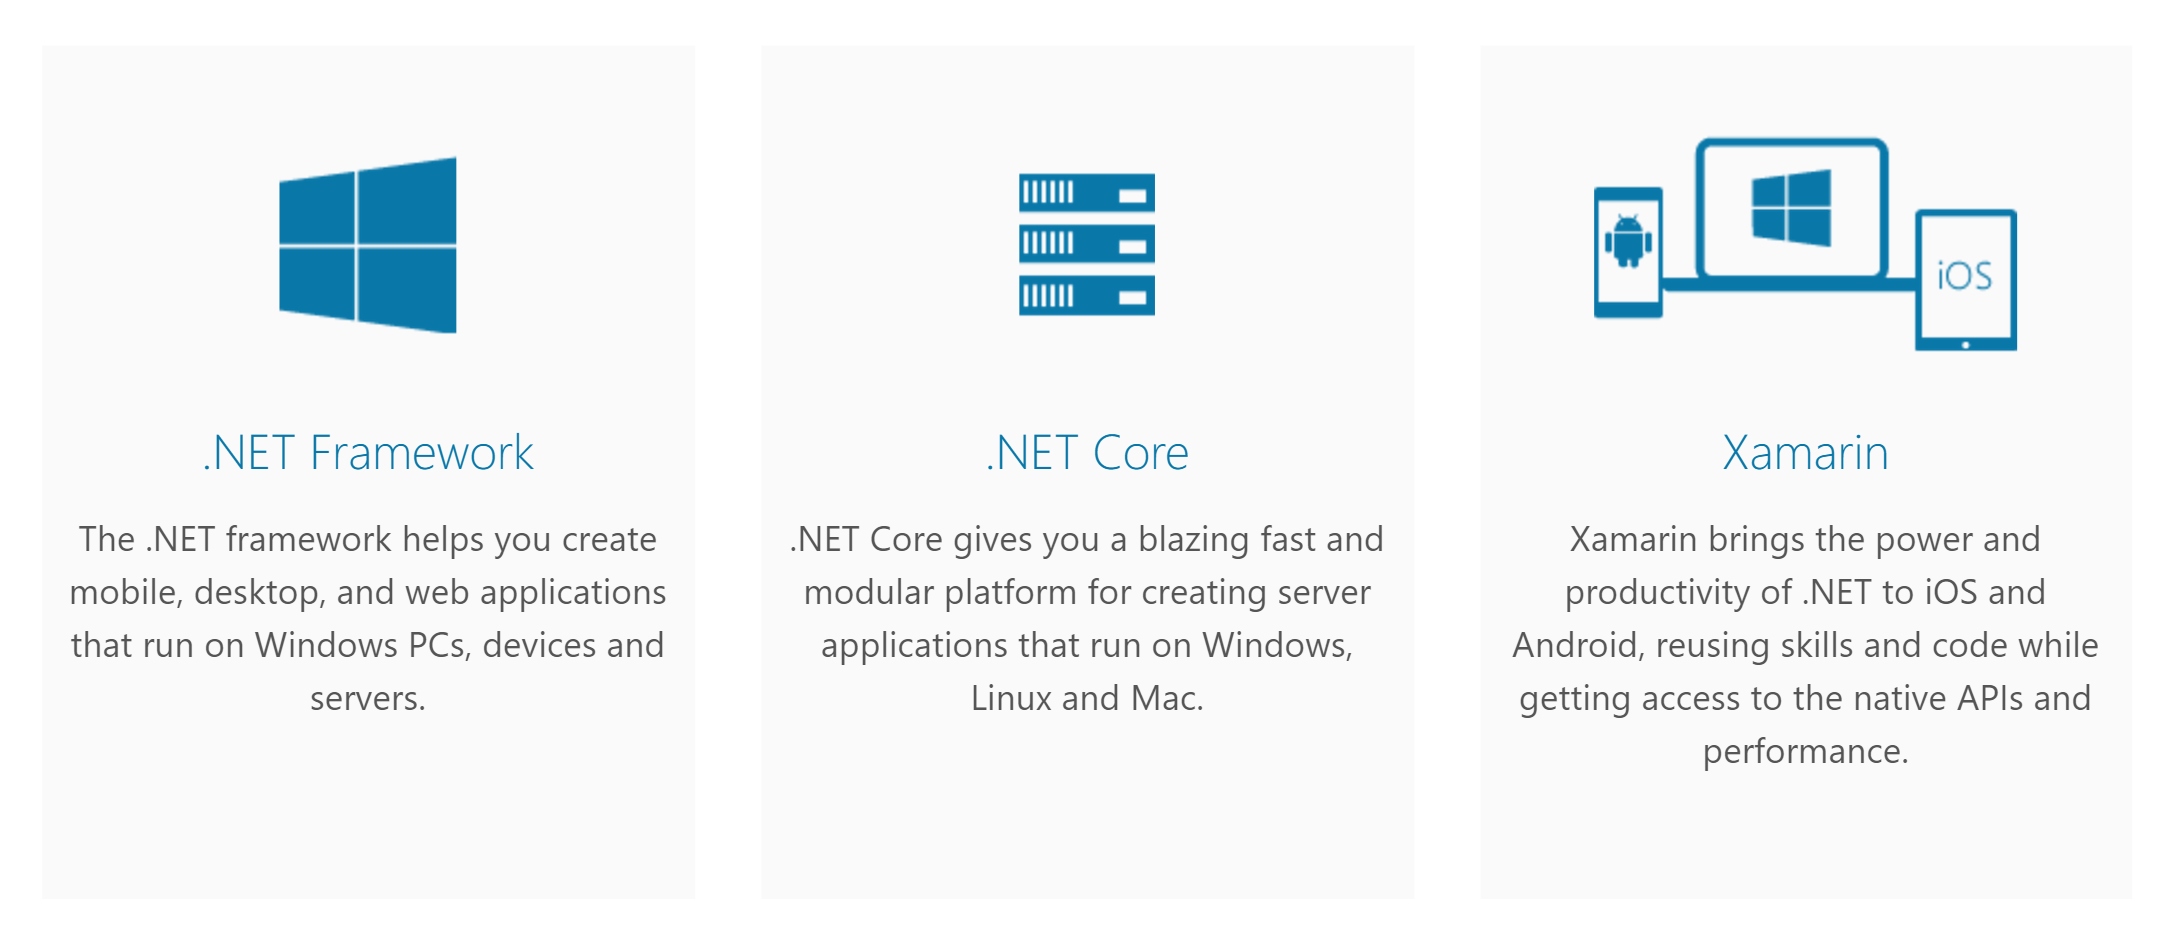
\includegraphics[width=0.8\textwidth]{net-ecosystem.png}
    \caption{.NET ecosystem}
\end{figure}

\subsection{Languages}

\begin{itemize}
    \item Syntax very similar to C, C++, Java \& JavaScript
    \item Functional programming language, cross-platform, open source
    \item Approachable English-like language for OOP
\end{itemize}

\subsection{Applications}

\begin{itemize}
    \item desktop
    \item web \& server
    \item mobile
    \item gaming
    \item IoT
    \item AI
\end{itemize}

\subsubsection{Desktop}

\begin{itemize}
    \item UWP (Universal Windows Project)
    \item Xamarin.Mac
    \item WPF (Windows Presentation Foundation)
    \item WinForms (Windows Forms)
\end{itemize}

\subsubsection{Web \& Server}
\begin{itemize}
    \item ASP.NET
    \item ASP.NET Core
\end{itemize}

\subsubsection{Mobile}
\begin{itemize}
    \item UWP (Universal Windows Project)
    \item Xamarin
\end{itemize}

\subsubsection{Gaming}
\begin{itemize}
    \item Unity
    \item CryEngine
\end{itemize}

\subsubsection{IoT}
\begin{itemize}
    \item UWP
    \item .NET Core IoT
\end{itemize}

\subsubsection{AI}

\begin{itemize}
    \item Cognitive Services
    \item Azure Machine Learning
    \item Machine Learning and AI Libraries
    \item F\# for Data Science and ML
\end{itemize}

\subsection{Xamarin}
\begin{itemize}
    \item `Target all platforms with a single, shared codebase for Android, iOS, Windows'. 
    \item Developen van Mobile devices lastig: verschillende platformen, verschillende talen voor elk device.
    \item Oplossing: Xamarin
    \item Extensie op Visual Studio.
\end{itemize}


\begin{figure}[H]
    \centering
    
\includegraphics[width=0.1\textwidth]{xamarin-logo.png}
    \caption{Xamarin Logo}
\end{figure}

\subsubsection{Xamarin - UI Technology}
\begin{figure}[H]
    \centering
    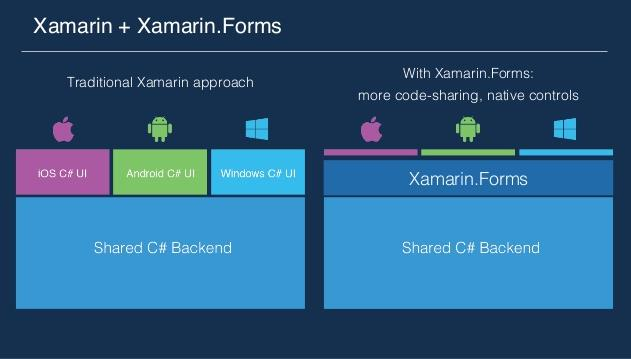
\includegraphics[width=0.7\textwidth]{xamarin-forms.png}
    \caption{Native vs Xamarin.Forms}
\end{figure}

\subsubsection{Xamarin - Code Sharing strategy}

\begin{figure}[H]
    \centering
    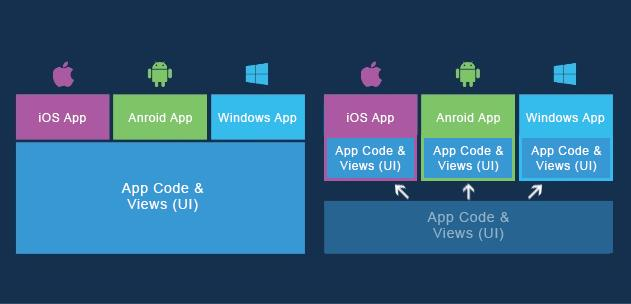
\includegraphics[width=0.7\textwidth]{xamarin-codesharing.png}
    \caption{.NET Standard vs Shared (Assets) Project}
\end{figure}

Met Shared Assets Project maken we de UI voor elk platform apart. Wij gaan vooral werken met .NET Standard.


\subsection{Vragen}

\begin{itemize}
    \item What devices, platforms, etc. can we target using .NET, and what programming languages can we use?
    \item What is the basic difference between .NET Standard and Shared Assets projects in Xamarin?
    \item What is the difference between Xamarin native and Xamarin.Forms? What are the advantages and disadvantages?
    \item How to set up and understand the structure of a Xamarin project for the labs in this course, and how to debug on the different platforms.
\end{itemize}

\section{C\# Syntax}

\subsection{Python vs C\#}

\begin{itemize}
    \item curly brackets \{ \} in plaats van indenting
\end{itemize}

\subsection{Datatypes}
\begin{figure}[H]
    \centering
    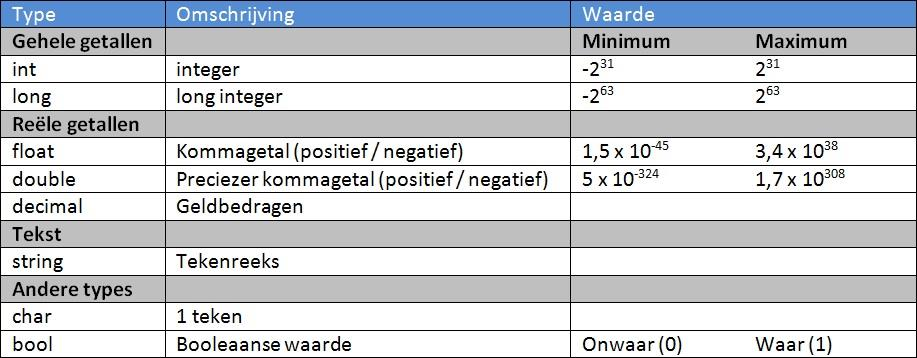
\includegraphics[width=0.5\textwidth]{csharp-datatypes.png}
    \caption{Datatypes in C\#}
\end{figure}

\subsection{Collections}
\begin{itemize}
    \item Array
    \item Dictionary<TKey, TValue>
    \item List<T>
\end{itemize}

Collection type = fixed! $\Rightarrow$ Je kan alleen objecten van het gekozen type toevoegen aan een collection

\begin{lstlisting}[language=csharp]
//collections of type Person:
Person[] teacherArr = new Person[10];
List<Person> teacherList = new List<Person>();

//You can only add Person objects to these collections!
\end{lstlisting}


\subsubsection{Arrays}
= meerdere variabelen van hetzelfde type

\begin{lstlisting}[language=csharp]
//initialize int array with 10 positions:
int[] numbers = new int[10];
//save number 13 in the first position
numbers[0] = 13;
//print the value of the first number in the array:
Debug.WriteLine("The first number is:" +numbers[0]);
//intialize and fill another array with 4 numbers:
int[] startPositions = { 4, 1, 9, 3 };
\end{lstlisting}

\subsubsection{Dictionary <TKey, TValue>}

\begin{lstlisting}[language=csharp]
//declare dictionary with key type & value type
Dictionary<string, int> studentScores = new Dictionary<string, int>();
//add two elements (key value pairs)
studentScores.Add("Jean-Jacques", 13);
studentScores.Add("Jean-Louis", 4);
//get the score of Jean-Jacques
int score = studentScores["Jean-Jacques"];
\end{lstlisting}


\subsubsection{List<T>}

\begin{lstlisting}[language=csharp]
//declare list, fill one by one:
List<string> emailList = new List<string>();
emailList.Add("stijn.walcarius@howest.be");
emailList.Add("frederik.waeyaert@howest.be");
//get elements out (two ways):
string first = emailList.ElementAt(0);
string second = emailList[1];
//declare + fill list:
List<string> teacherList = new List<string> { "SWC", "FWA" };
\end{lstlisting}

\subsection{Selections}
if / else if / else / switch

\begin{lstlisting}[language=csharp]
if(findTheoryTeacher == true) {
    email1 = "frederik.waeyaert@howest.be";
    email2 = null;
}
else if(findLabTeachers == true) {
    email1 = "stijn.walcarius@howest.be";
    email2 = " frederik.waeyaert@howest.be";
} else {
    email1 = email2 = null;
}
\end{lstlisting}

\begin{lstlisting}[language=csharp]
switch (teacher){
    case "SWC":
        email = "stijn.walcarius@howest.be";
        break;
    case "FWA":
        email = "frederik.waeyaert@howest.be";
        break;
    default:
        email = "info@howest.be";
        break;
}
\end{lstlisting}

\subsection{Loops}
for / foreach / while / do while

\begin{lstlisting}[language=csharp]
for(int i = 0; i < 100; i++) {
    //do something 100 times
}
\end{lstlisting}

\begin{lstlisting}[language=csharp]
List<string> teacherList = new List<string> { "SWC", "FWA" };
foreach(string teacher in teacherList) {
    //do something
}
\end{lstlisting}

\begin{lstlisting}[language=csharp]
while(endOfClass == false){
    //might never be executed
}
\end{lstlisting}

\begin{lstlisting}[language=csharp]
do {
    //executed at least once!
} while(endOfClass == false);
\end{lstlisting}

\subsection{Classes}
\begin{lstlisting}[language=csharp]
public class Person
{
    //property
    public string Name { 
        get {...};
        set {...}; 
    }

    //constructor
    public Person(string name) {
        this.Name = name;
    }

    //method
    public void Subscribe() {
        //do something
    }
}
\end{lstlisting}

\subsection{Instantiate objects}

\begin{lstlisting}[language=csharp]
Persons p1 = new Person("Stijn");

// Based on the following constructor in the Person class:
public Person (string name) {
    this.Name = name;
}
\end{lstlisting}

\subsection{Properties}

\subsubsection{Fields vs properties}

\begin{itemize}
    \item Fields store the actual data
    \item Properties are used to access those fields
    \item Auto-implemented properties have a hidden field
    \item Use properties to control field access
    \item Enhance input/output control using get \& set
    \item Calculated properties build on other properties
    \begin{itemize}
        \item No field required
        \item Reusability
    \end{itemize}
\end{itemize}

\begin{lstlisting}[language=csharp]
//private field
private int _id;

//property (zetten we altijd public)
public int Id {
    // getter
    get { return _id; }
    // setter
    set { _id = value; }
}
\end{lstlisting}


\subsubsection{Default values for properties}

\begin{itemize}
    \item Setting default values can be useful
    \item Default values can be set\dots
    \begin{itemize}
        \item \dots with full properties
        \item \dots with auto-implemented properties
        \item \dots in the constructor
    \end{itemize}
\end{itemize}

\subsection{Constructor}

\begin{itemize}
    \item A constructor is called every time you create an instance of a class
    \item It is used to allow / force the user to provide certain values
    \item Default constructor is (only) added if a model has no constructors
    \item Constructor overloading = multiple constructors with either \dots
    \begin{itemize}
        \item \dots a different number of parameters, or
        \item \dots a different type of paramters, or
        \item \dots the same parameters in a different order
    \end{itemize}
    \item Constructors should call each other for enhanced efficiency
    \item Constructors in inheriting classes call the constructors of the base class
\end{itemize}


\end{document}